% 第 11 题图丙：坐标纸（a-n 网格，供学生描点绘图）
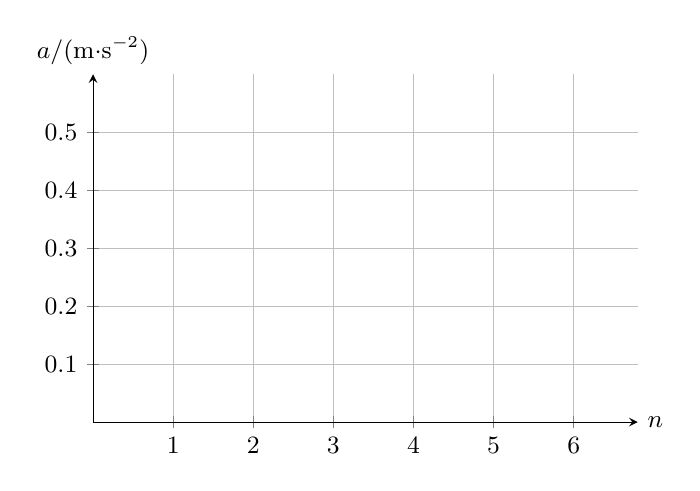
\begin{tikzpicture}[font=\small]
  \begin{axis}[
      width=8.5cm, height=6cm,
      axis lines=middle, grid=both, minor grid style={gray!40},
      xlabel={$n$}, ylabel={$a$/(m$\cdot$s$^{-2}$)},
      xmin=0, xmax=6.8, ymin=0, ymax=0.6,
      xtick={1,2,...,6}, ytick={0.1,0.2,...,0.5},
      xlabel style={anchor=west}, ylabel style={anchor=south}, font=\small]
  \end{axis}
\end{tikzpicture}
